%%
%% This is file `sample-authordraft.tex',
%% generated with the docstrip utility.
%%
%% The original source files were:
%%
%% samples.dtx  (with options: `authordraft')
%% 
%% IMPORTANT NOTICE:
%% 
%% For the copyright see the source file.
%% 
%% Any modified versions of this file must be renamed
%% with new filenames distinct from sample-authordraft.tex.
%% 
%% For distribution of the original source see the terms
%% for copying and modification in the file samples.dtx.
%% 
%% This generated file may be distributed as long as the
%% original source files, as listed above, are part of the
%% same distribution. (The sources need not necessarily be
%% in the same archive or directory.)
%%
%% The first command in your LaTeX source must be the \documentclass command.
\documentclass[sigconf,authordraft]{acmart}
\usepackage{graphicx}

%%
%% \BibTeX command to typeset BibTeX logo in the docs
\AtBeginDocument{%
  \providecommand\BibTeX{{%
    \normalfont B\kern-0.5em{\scshape i\kern-0.25em b}\kern-0.8em\TeX}}}

%% Rights management information.  This information is sent to you
%% when you complete the rights form.  These commands have SAMPLE
%% values in them; it is your responsibility as an author to replace
%% the commands and values with those provided to you when you
%% complete the rights form.
%%\setcopyright{acmcopyright}
%%\copyrightyear{2018}
%%\acmYear{2018}
%%\acmDOI{10.1145/1122445.1122456}

%% These commands are for a PROCEEDINGS abstract or paper.
%%\acmConference[Woodstock '18]{Woodstock '18: ACM Symposium on Neural
%%  Gaze Detection}{June 03--05, 2018}{Woodstock, NY}
%%\acmBooktitle{Woodstock '18: ACM Symposium on Neural Gaze %%Detection,
%%  June 03--05, 2018, Woodstock, NY}
%%\acmPrice{15.00}
%%\acmISBN{978-1-4503-9999-9/18/06}

%%
%% Submission ID.
%% Use this when submitting an article to a sponsored event. You'll
%% receive a unique submission ID from the organizers
%% of the event, and this ID should be used as the parameter to this command.
%%\acmSubmissionID{123-A56-BU3}

%%
%% The majority of ACM publications use numbered citations and
%% references.  The command \citestyle{authoryear} switches to the
%% "author year" style.
%%
%% If you are preparing content for an event
%% sponsored by ACM SIGGRAPH, you must use the "author year" style of
%% citations and references.
%% Uncommenting
%% the next command will enable that style.
%%\citestyle{acmauthoryear}

%%
%% end of the preamble, start of the body of the document source.
\begin{document}

%%
%% The "title" command has an optional parameter,
%% allowing the author to define a "short title" to be used in page headers.
\title{Gene Network Modelling: \\ Improved Gene Co-Expression Network Clustering}

%%
%% The "author" command and its associated commands are used to define
%% the authors and their affiliations.
%% Of note is the shared affiliation of the first two authors, and the
%% "authornote" and "authornotemark" commands
%% used to denote shared contribution to the research.
\author{Nathan Dale S. Paglinawan}
\authornote{Both authors contributed equally to this research.}
%%\orcid{1234-5678-9012}
\author{Micah G. Tan}
\authornotemark[1]
\email{nathandale.paglinawan@gmail.com}
\email{micah.tan97@gmail.com}
\affiliation{%
  \institution{Algorithms and Complexity Laboratory}
  \institution{Department of Computer Science}
  \institution{University of the Philippines Diliman}
  \city{Diliman, Quezon City}
  \state{National Capital Region}
  \country{Philippines}
  \postcode{1101}
}

%%
%% By default, the full list of authors will be used in the page
%% headers. Often, this list is too long, and will overlap
%% other information printed in the page headers. This command allows
%% the author to define a more concise list
%% of authors' names for this purpose.
\renewcommand{\shortauthors}{Paglinawan and Tan}

%%
%% The abstract is a short summary of the work to be presented in the
%% article.
\begin{abstract}
    Gene networks are an effective way to illustrate on how genes interact with each other, because genes rarely work on their own. One example is the gene co-expression network, which can be used to identify which genes are responsible for the manifestation of a phenotype, such as a physical trait, or a disease.
    
    WGCNA is a widely used tool to construct and analyze gene co-expression networks. It uses a hierarchical clustering (HC) mechanism to create clusters. However, despite its popularity, it still has shortcomings. One research sought to improve WGCNA by implementing a hybrid of HC and k-means clustering, in an attempt to address its drawbacks. However, it only dealt with WGCNA's static modelling. It was still susceptible to: a.) sensitivity to noise and outliers; b.) breaking large clusters; and c.) difficulty handling different sized clusters and convex shapes. Looking through other clustering algorithms, we found a clustering method that deals with these problems. 
    
    In this study, we propose to use Density-Based Spatial Clustering of Applications with Noise (DBSCAN) as an alternative clustering mechanism to standard WGCNA's HC in an attempt to improve its accuracy. If successful, this will open up a better alternative add-on to improve the clustering mechanism of WGCNA, as well as improve gene network modelling as a whole. This will also facilitate improved identification of genes related to the manifestation of deadly diseases such as cancer, which will assist in the prognosis, early detection, and open up avenues in finding new cures and treatments against such diseases.
    
    The statistical test results showed some promise in improving accuracy of the clustering mechanism of WGCNA. However, further development of a systematic method for defining parameters of DBSCAN is recommended to address the slow running time, and to achieve a higher accuracy rating.
\end{abstract}

%%
%% The code below is generated by the tool at http://dl.acm.org/ccs.cfm.
%% Please copy and paste the code instead of the example below.
%%
\begin{CCSXML}
<ccs2012>
<concept>
<concept_id>10010405.10010444.10010095</concept_id>
<concept_desc>Applied computing~Systems biology</concept_desc>
<concept_significance>500</concept_significance>
</concept>
<concept>
<concept_id>10010405.10010444.10010450</concept_id>
<concept_desc>Applied computing~Bioinformatics</concept_desc>
<concept_significance>500</concept_significance>
</concept>
</ccs2012>
\end{CCSXML}

\ccsdesc[500]{Applied computing~Systems biology}
\ccsdesc[500]{Applied computing~Bioinformatics}

%%
%% Keywords. The author(s) should pick words that accurately describe
%% the work being presented. Separate the keywords with commas.
\keywords{bioinformatics, gene networks, gene co-expression networks, gene correlation networks, accuracy, WGCNA, clustering, hierarchical clustering, k-means clustering, DBSCAN, module detection, DNA microarray data, yeast cell cycle dataset, gene expression data simulation, statistical testing, Rand Index, Jaccard Coefficient, Similarity Index}

%%
%% This command processes the author and affiliation and title
%% information and builds the first part of the formatted document.
\maketitle

\section{Introduction}
Chromosomes, which can be found in the nucleus of most living cells, are made up of genes. These genes carry information, instructions for the synthesis of proteins in cells that is used during gene expression. Gene expression is the generation of a functional gene product, which are often proteins, from the information encoded by a gene \cite{na001}. These proteins determine the structure and function of the cells, which are responsible for the manifestation of physical characteristics or diseases. However, genes rarely operate on their own. They are interconnected as a network. Oftentimes, it takes more than one gene to be expressed for a phenotype, such as a physical trait, or a disease, to be manifested. Studies have shown that each gene is estimated on average to interact with four to eight other genes and to be involved in 10 biological functions \cite{Li2018}. Gene networks play a big role in identifying which genes are associated with complex human diseases such as cancer, which could serve as promising starting points of researching potential cures and treatments for these diseases. Constructing a gene co-expression network is an effective way to characterize the correlation patterns among genes \cite{Li2018}. A gene co-expression network is an undirected graph, where each node corresponds to a gene, and each edge connects a pair of genes that are significantly correlated \cite{Li2018}.

Weighted gene co-expression network analysis (WGCNA) is a widely used tool to construct and analyze gene co-expression networks, that can be utilized for finding clusters (modules) of highly correlated genes (i.e. hub genes / highly connected network genes) \cite{LangfelderHorvath2008}. Correlation networks facilitate network based gene screening methods that can be used to identify candidate biomarkers or therapeutic targets \cite{LangfelderHorvath2008}. Improving the accuracy of the clustering mechanism of WGCNA could allow for better classification of gene functions, and subsequently, for a better identification and understanding of genes that are related to diseases. 

\section{Theoretical Framework}
Gene co-expression networks are built on the basis of a gene co-expression measure. The network nodes correspond to genes or more precisely, to gene expression profiles. The \textit{ith} gene expression profile $x_i$ is a vector whose components report the gene expression values across \textit{m} microarrays. We define the co-expression similarity $s_{ij}$ between genes i and j as the absolute value of the correlation coefficient between their expression profiles: \\ 
(Equation 1) $s_{ij} = |$cor$(x_i,x_j)|$ \\
Using a thresholding procedure, this co-expression similarity is transformed into a measure of connection strength (adjacency). An unweighted network adjacency $a_{ij}$ between gene expression profiles $x_i$ and $x_j$ can be defined by hard thresholding the co-expression similarity $s_{ij}$ as follows: \\
(Equation 2) $s_{ij}=$
\begin{cases}
1, & \text{if } $s_{ij}$ $\geq$ $\tau$ \\
0, & \text{otherwise}
\end{cases} \\
where $\tau$ is the "hard" threshold parameter. Thus, two genes are linked $(a_{ij}=1)$ if the absolute correlation between their expression profiles exceeds the (hard) threshold $\tau$. 

Hard thresholding of the correlation leads to simple network concepts (e.g. the gene connectivity equals the number of direct neighbors), but it may lead to a loss of information: if $\tau$ has been set to 0.8, there will be no link between two genes if their correlation equals 0.799. 

To preserve the continuous nature of the co-expression information, one could simply define a weighted adjacency matrix as the absolute value of the gene expression correlation matrix, i.e., $[a_{ij}]=[s_{ij}]$ . However, since microarray data can be noisy and the number of samples is often small, we and others have found it useful to emphasize strong correlations and to punish weak correlations. It is natural to define the adjacency between two genes as a power of the absolute value of the correlation coefficient \cite{ZhangHorvath2005},\cite{HorvathZhangEtal2006}: \\
(Equation 3) $a_{ij}=s_{ij}^{\beta}$ with $\beta \geq 1$ \\
This soft thresholding approach leads to a weighted gene co-expression network.

The adjacency in Equation 3 implies that the weighted adjacency $a_{ij}$ between two genes is proportional to their similarity on a logarithmic scale, $log(a_{ij}) = \beta log(s_{ij})$. Adjacency functions for both weighted and unweighted networks require the user to choose threshold parameters, for example by applying the approximate scale-free topology criterion \cite{YipHorvath2007}.

Once the network has been constructed, module detection is often a logical next step. Modules are defined as clusters of densely interconnected genes \cite{LangfelderHorvath2008}. The network and modules can be interrogated to identify regulators, functional enrichment and hub genes. Differential co-expression analysis can be used to identify modules that behave differently under different conditions.Potential disease genes can be identified using a Guilt-By-Association (GBA) approach that highlights genes that are co-expressed with multiple disease genes \cite{vanDamEtal2017}.

\section{Related Work}

In bioinformatics applications, correlation networks are increasingly being utilized. Langfelder and Horvath \cite{LangfelderHorvath2008} made an implementation of Weighted Gene Co-expression Network (WGCNA) in R which is one of the most used programs for gene co-expression network. Their paper presented limitations for WGCNA which are: a.) WGCNA assumes that the microarray data has been properly pre-processed and normalized: b.) The results of WGCNA can be biased or invalid when dealing with technical artefacts, tissue contaminations, or poor experimental design; c.) Although several co-expression module detection methods are implemented, the package does not provide means to determine which method is best; and d.) The WGCNA R package is limited to undirected networks. For this research we focused on the limitations of WGCNA in co-expression module detection.

In the package, hierarchical clustering (HC) was used as a detection method. In HC the objects are joined together in a hierarchical fashion from the closest, that is most similar, to the furthest apart, that is the most different \cite{Greenacre2008}. Karypis et al. \cite{KarypisEtal1999} discussed how based on the type of distance matrix chosen for merging different algorithms can suffer from one or more of the following: a.) sensitivity to noise and outliers; b.) breaking large clusters; and c.) difficulty handling different sized clusters and convex shapes. The merging decisions are based upon static modeling of the clusters to be merged. Also, the merging decisions of hierarchical clustering are based upon static modeling of the clusters to be merged. This means that once a gene falls under a subdendrogram, this decision cannot be modified.

To address the weaknesses of HC, Bot\'{i}a et al. \cite{BotiaEtal2017} implemented a hybrid of HC and k-means clustering. K-means clustering aims to divide the points in the dimension into k clusters so that the within-cluster sum of squares is minimized \cite{HartiganWong1979}. In the hybrid, k-means will move genes between modules thus effectively undoing premature decisions made by HC when assigning genes to sub-dendrograms. It also takes advantage of HC to carry out sensible initialization. The value of $k$ is equal to the number of modules discovered by HC and the centroids are initialized to the eigengenes generated by WGCNA \cite{BotiaEtal2017}.

Although the hybrid method addresses the static modeling of HC, it still suffers from: a.) sensitivity to noise and outliers; b.) breaking large clusters; and c.) difficulty handling different sized clusters and convex shapes. A clustering method which deals with these problems is Density-Based Spatial Clustering of Applications with Noise (DBSCAN) \cite{EsterEtal1996}. 

DBSCAN is a density based clustering algorithm wherein given a set of points in some space, it groups together points that are closely packed together (points with many nearby neighbors), and it marks as outliers the points that lie alone in low-density regions (whose nearest neighbors are too far away) \cite{EsterEtal1996}. But before DBSCAN can proceed, 2 parameters need to be specified, namely, $MinPts$ and $\varepsilon$. $MinPts$ is the minimum number of data points needed to determine a single cluster. $\varepsilon$ is the radius given to test the distance between data points. If a point falls within the epsilon distance of another point, those two points will be in the same cluster \cite{Lutins2017}. DBSCAN can find arbitrarily shaped clusters. It can even find a cluster completely surrounded by a different cluster. It also reduces the so called single-link effect. DBSCAN has a notion of noise, and is robust to outliers. Also, it does not require one to specify the number of clusters in the data a priori, as opposed to k-means. Kotsiantis and Pintelas \cite{KotsiantisandPintelas2004} also mentions that DBSCAN is much faster than hierarchical clustering algorithms and partitioning algorithms, such as k-means clustering. In this study, we propose to use DBSCAN as an improvement to the HC mechanism of standard WGCNA.

\section{Problem Statement}

This study aims to answer the following questions:
\begin{itemize}
	\item Is there a way to improve the accuracy of WGCNA, particularly its clustering mechanism?

	\item How can the accuracy of the different variants (HC, HC + k-means hybrid, DBSCAN) of the clustering mechanism of WGCNA be measured and compared?
\end{itemize}

\section{Significance of the study}

This study aims to open up a better, more accurate alternative method to improve the clustering mechanism of WGCNA, as well as improve gene network modelling as a whole. This will facilitate more accurate identification of genes related to the manifestation of deadly diseases such as cancer, which will assist in the prognosis, early detection, and opening up of avenues in finding new cures and treatments against such diseases.

\section{Objectives of the Study}

The main objectives of this study are as follows:
\begin{itemize}
	\item Develop an improvement to the accuracy of the clustering mechanism of WGCNA.

	\item Devise metrics for measuring and comparing the accuracy of the different variants (HC, HC + k-means hybrid, DBSCAN) of clustering mechanisms of WGCNA.

\end{itemize}

\section{Scope and Limitations of the Study}

This study will focus only on improving the clustering mechanism of, and not the whole WGCNA process. This study will be using a yeast cell cycle data, as described in \cite{ChoEtal1998}, acquired from the Yeast Cell Cycle Analysis Project \cite{SpellmanEtal1998}, which is classified as DNA microarray data.

\section{Methodology}

\subsection{Data and Data Preprocessing}
The data used is the yeast cell cycle data, as described in \cite{ChoEtal1998}, acquired from the Yeast Cell Cycle Analysis Project \cite{SpellmanEtal1998}, which is classified as DNA microarray data. The data contained 6179 rows, 6178 correspond to the genes and 1 corresponds to the column names, and 83 columns, 82 correspond to the samples and 1 corresponds to the row names. We remove unnecessary columns, i.e. columns that act as data separators and contain no data, resulting to 6179 rows, and 78 columns. Taking note that WGCNA requires an input wherein the rows are the samples and the columns are the genes, we transpose the data and properly name the rows and columns, using the values in the first column and values in the first row, respectively, yielding 77 columns, which are the samples, and 6718, which are the genes. Observing that there are some missing values in the data, we filled up the missing values using mean imputation, which is computed by getting the average value of the available, i.e. not missing, values in a column, and using that computed value to fill up the missing values in that particular column. Mean imputation is one of the most commonly used methods in filling up missing data, because it does not affect the distribution of the data values, it does not create outliers in the data, and it uses the expected value, i.e. mean, to fill up the missing data.

\subsection{Matrix Construction}
WGCNA \cite{LangfelderHorvath2008} constructs two matrices. To fit the degree distribution in a small-word network, it first defines a correlation matrix up to a power $\beta$ . This matrix gives information about the expression correlation between genes.

In detail, the correlation data was transformed to an adjacency matrix using the formula: $a_{ij}=(s_{ij},\beta) =|s_{ij}|$ , where $\beta$ represents the exponential parameter for a power law distribution. In general, the number of connections of all the genes in a scale-free network follow a power law distribution $P(k)$ \texttildelow  $k-\beta$. The $P(k)$ in our co-expression network indicates the probability that a gene is co-expressed with k other genes. By setting the criterion that the co-efficiency of $log(k)$ and $log(p(k))$ is greater than 0.8, we checked all the possible values of $\beta$ \cite{HorvathZhangEtal2006}.

    
WGCNA thinks that co-expression is not enough, and that the similarity between genes should be reflected at the expression and the network topology level. To further identify functional modules, another adjacency matrix that considers topological similarity was constructed. This was done by transforming the adjacency matrix to a topological overlap matrix (TOM) using WGCNA package. This step alleviates the effect of noisy genes when obtaining the adjacency from the correlation \cite{YipHorvath2007}. 

Normally, the TOM matrix is the final matrix of WGCNA, but once the network is built through the TOM, it is converted to a dissimilarity matrix $(1-TOM)$ which is used as the basis for clustering. 

\subsection{Clustering and Module Detection}
WGCNA uses a hierarchical clustering (HC) mechanism to create clusters. However, despite its popularity, it still has shortcomings. One research sought to improve WGCNA by implementing a hybrid of HC and k-means clustering, in an attempt to address its drawbacks. However, it only dealt with WGCNA's static modelling. It was still susceptible to: (1) sensitivity to noise and outliers; (2) breaking large clusters; and (3) difficulty handling different sized clusters and convex shapes. Looking through other clustering algorithms, we found a clustering method that deals with these problems. In this study, we use Density-Based Spatial Clustering of Applications with Noise (DBSCAN) as an alternative clustering mechanism to standard WGCNA's HC in an attempt to improve its accuracy.

\subsubsection{Hierarchical Clustering}
WGCNA provides a module for hierarchical clustering which step by step merges the current pair of mutually closest nodes into a new node until there is one final node remaining, which comprises the entire data set. Hierarchical clustering first looks for the pair of samples that are most similar, which is the closest in the sense of having the lowest dissimilarity. These two samples are then joined at the level of their dissimilarity in the first step of the dendrogram, or clustering tree. The point at which they are joined is called a node. The dissimilarity is then calculated between the merged pair and the other samples. This process is done repeatedly until there is only one node left. 
After clustering the samples, it then goes through the process of module detection. Standard WGCNA uses an R package called Dynamic Tree Cut. Dynamic Tree Cut accepts a minimum module size, which we set to 30, a relatively high size value to make large modules \cite{Greenacre2008}.

\subsubsection{K-means Clustering}
K-means clustering measures cluster similarity with regards to the mean value of the objects in a cluster, which can be viewed as the cluster's centroid or center of gravity. In the additional k-means clustering paper, the eigengenes were used as centroids. Due to time constraints, using the same method was not possible so instead, we used the built in k-means function in R \cite{RLanguageEnvironment} which accepts a number of centers as input. The resulting number of clusters from hierarchical clustering was used as the input.

Because no centroids were given, k-means randomly generates cluster centers according to the given input. Once all cluster centers are established, each point is assigned to the clusters based on the minimum distance to the cluster center. The cluster centers are then updated based on the points assigned to them. The center of mass of each cluster can be found by getting the sum of all the points and dividing by the total number of points. The resulting center of mass for each cluster is now the new cluster center. These steps are then repeated, iterating between assigning points to cluster centers, and updating the cluster centers until it reaches convergence \cite{AliKadhum2017}.

\subsubsection{Density-based Spatial Clustering with Noise}
In DBSCAN, there are two kinds of points in a cluster, points inside of the cluster (core points) and points on the border of the cluster (border points). These points are computed based on having at least a given number of neighboring points ($minPts$) in a given radius ($\varepsilon$). To find a cluster, DBSCAN starts with an arbitrary point $p$ and retrieves all points density-reachable from $p$ with respect to $minPts$. If $p$ is a core point, this procedure yields a cluster with respect to $minPts$ and $\varepsilon$. If $p$ is a border point, no points are density-reachable from $p$, and DBSCAN visits the next point of the database. This is done until all points are reached. 

At present, there is no systematic way for determining a value for $minPts$. As an alternative, we implement DBSCAN with different values of $minPts$ within the range of 5 to 100 with an increment of 5.

To find the value of $\varepsilon$ we compute the k-nearest neighbor distances in a matrix of points. We calculate the average of the distances of every point to its nearest $k$ neighbors. The value of corresponds to $minPts$. These k-distances are plotted in an ascending order to determine the knee. A knee corresponds to a threshold where a sharp change occurs along the k-distance curve. This knee will be the parameter \cite{EsterEtal1996}.

\subsection{Gene Expression Data Simulation}
In testing for accuracy, (i.e. Gene Expression Data Simulation and Statistical Testing), we followed the pipeline of the researchers of the additional k-means step to the clustering mechanism of WGCNA \cite{BotiaEtal2017}. We wanted to measure and compare the accuracy of the different variants (HC, HC + K-means hybrid, DBSCAN) of the clustering mechanism of WGCNA. The WGCNA package has a built in function called $simulateDatExpr()$ \cite{LangfelderHorvath2008}, which is a convenient method for simulating artificial  gene co-expression data sets based on the eigengene of the gene expression for each gene belonging to the modules.

The data simulation process requires the following arguments \cite{LangfelderHorvath2008}: (1) a data frame containing the module eigengenes to be used to seed for the simulated modules. Rows correspond to samples and columns correspond to modules; (2) a numeric vector containing the proportions of the total number of genes to be put into each of the modules, i.e. the module partition/assignment; and (3) the total number of genes to be simulated. 

The data simulation process returns the following \cite{LangfelderHorvath2008}: (1) a data frame containing the simulated expression data, let us denote it as $D$, whose columns correspond genes and rows to samples; and (2) a numeric vector containing the simulated module assignment, which is also the ideal/theoretical optimal clustering partition of the simulated gene expression profile, let us denote it as $P(D)$.

Relying on the effectiveness of this simulation process, then a simulated data set $D$, we will prefer a GCN constructing algorithm $A$ over algorithm $B$ if the distance between $A(D)$ and $P(D)$ is smaller than between $B(D)$ and $P(D)$, where $A(D)$ and $B(D)$ are the clustering partitions resulting from constructing GCNs using $D$ with $A$ and $B$, respectively. The accuracy of an algorithm $A$ is defined by the similarity of the ideal/theoretical optimal partition of the simulated data to the partition constructed by $A$ \cite{BotiaEtal2017}.

In order to test whether the accuracy of the different variants (HC, HC + K-means hybrid, DBSCAN) of the clustering mechanism of WGCNA, we constructed a plausible set of simulated gene expression profiles. We used the yeast cell cycle data standard WGCNA GCNs (i.e. eigengenes and module partition/assignment) as the simulation seed for the generation of a simulated gene expression profile. 

The data simulation process produced a gene expression profile and a theoretical ideal clustering partition for the profile. We used this theoretical ideal partition to evaluate the accuracy of standard WGCNA, k-means, and DBSCAN. 

\subsection{Statistical Testing}

To estimate accuracy we use three different statistics: (1) the Rand index; (2) the Jaccard coefficient; and (3) the similarity index, all of them are implemented within the clv R package \cite{clvPackage}.

The variables $SS, SD, DS, DD$, which are needed for the calculation of the three aforementioned statistics, are defined as follows \cite{clvPackage}:

\begin{itemize}
	\item Given a pair of input vectors which contains information about two different partitionings (let say $U$ and $V$) of the same data set $X$.

	\item We refer to a pair of points $x_i$, $x_j$ (we assume that $i $ $!=$ $j$) from the data set using the following terms:
	
	\item $SS$ = number of pairs where both points belong to the same cluster in both partitionings $U$ and $V$.
	
	\item $SD$ = number of pairs where both points belong to the same cluster in partitioning $U$ but not in $V$.
	
	\item $DS$ = number of pairs where both points belong to the same cluster in partitioning $V$ but not in $U$.
	
	\item $DD$ = number of pairs where both points belong to different clusters in both partitionings $U$ and $V$.
\end{itemize}

The three aforementioned statistics are defined as follows \cite{clvPackage}:

The Rand Index is defined as: \[R = \frac{SS+DD}{SS+SD+DS+DD}\] The Rand Index is a measure of the similarity between two data clusterings. Since the denominator is the total number of pairs, the Rand Index represents the frequency of occurrence of agreements over the total pairs.

The Jaccard Coefficient is defined as: \[J = \frac{SS}{SS+SD+DS}\] The Jaccard Coefficient is used for gauging the similarity and diversity of sample sets. The Jaccard Coefficient is also known as the Intersection over Union.

The Similarity Index is defined as:
\[S(U,V) = \frac{A(U,V) - 1}{N-1}\] where N is the number of partitioned objects. The Similarity Index based on the confusion matrix is the measure which estimates how those two different partitionings, coming from one dataset, are different from each other. Let $M$ be a confusion matrix for partitionings $U$ and $V$. Any one to one function $\Sigma :\{1, 2, ... , n\} \rightarrow \{1, 2, ... , m\}$ is called an assignment or association. Using a set of assignment functions $A(U,V)$ defined as $A(U,V) = max\{sum(\forall\ i\ in\ length:($\Sigma$)), M[i,\Sigma(i)]}$ is found.

\section{Results and Discussion}

The following figure is a graph used to determine the soft thresholding power:

\begin{figure}[H]
\centering
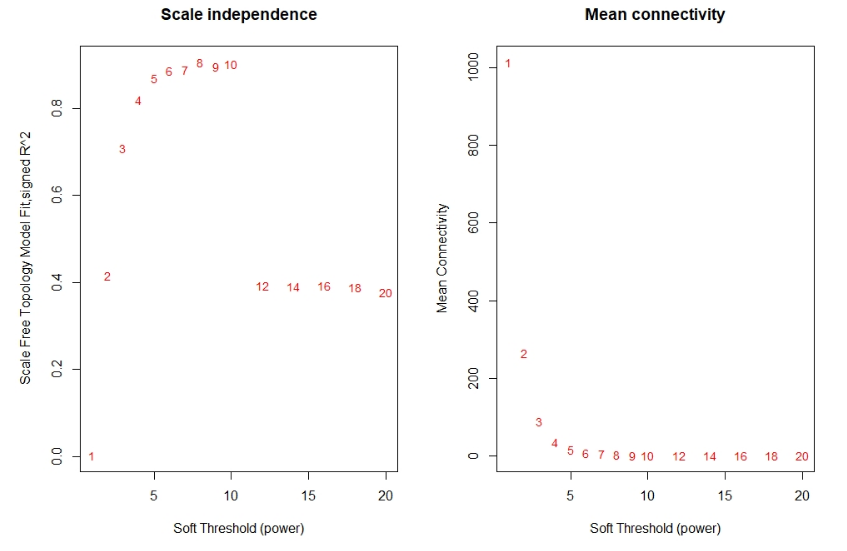
\includegraphics[scale=0.375]{Images/soft-thresholding.PNG}
\caption{Analysis of network topology for various soft-thresholding powers. a) The scale-free fit index (y-axis) as a function of the soft-thresholding power (x-axis). b) The mean connectivity (y-axis) as a function of the soft-thresholding power (x-axis).}
\end{figure}

In figure 1, we chose the power of value 5, which is the lowest power for which the scale-free topology fit index curve flattens out upon reaching a high value (in this case, roughly 0.90).

The following figure is a graph used to determine the value of $\varepsilon$:
\begin{figure}[h]
\centering
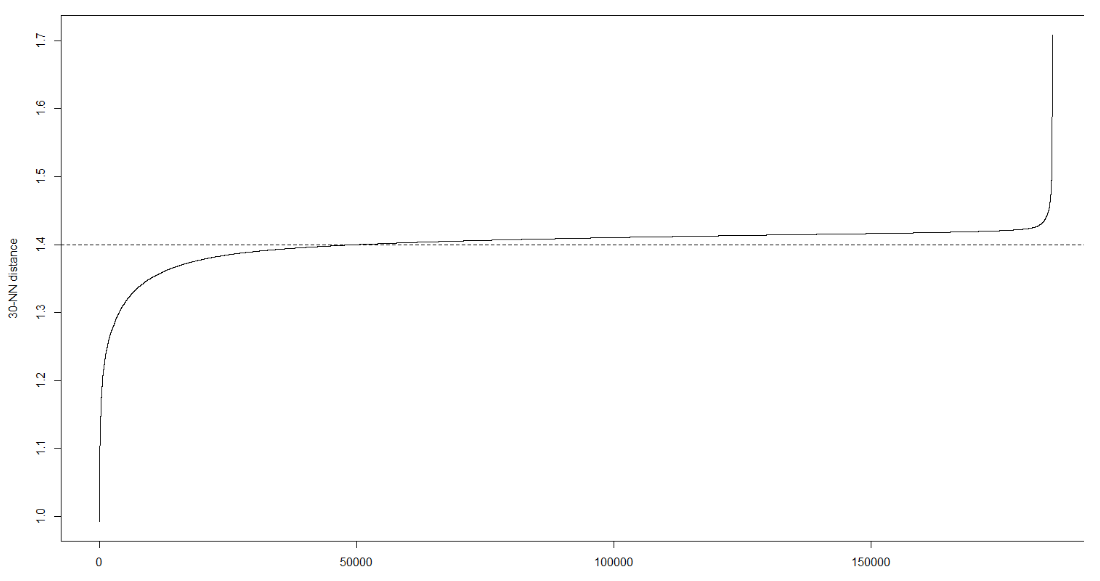
\includegraphics[width=8cm, height=6cm]{Images/knn-distance-plot.PNG}}
\caption{K-nearest neighbor distances (y-axis) in a matrix of points (x-axis).}
\end{figure}

In figure 2, we choose $\varepsilon$ to be 1.4 as seen in the graph in which a sharp turn occurred along the k-distance curve.

The clustering methods and simulated data produced the following partitions:
\begin{table}[H]
\begin{center}
\begin{tabular}{|c|c|c|c|c|c|c|c|c|c|c|}
\hline
\multicolumn{11}{|c|}{Hierarchical Clustering} \tabularnewline
\hline
0 & 1 & 2 & 3 & 4 & 5 & 6 & 7 & 8 & 9 & 10\\
\hline
751 & 929 & 871 & 801 & 408 & 383 & 354 & 163 & 161 & 153 & 152\\
\hline
\end{tabular}
\end{center}

\begin{center}
\begin{tabular}{|c|c|c|c|c|c|c|c|c|c|c|c|}
\hline
11 & 12 & 13 & 14 & 15 & 16 & 17 & 18 & 19 & 20 & 21 & 22\\
\hline
132 & 132 & 125 & 107 & 94 & 82 & 80 & 76 & 74 & 59 & 52 & 39\\
\hline
\end{tabular}
\end{center}
\caption{The number of genes in each module produced by Hierarchical Clustering. The label 0 is reserved for genes outside of all modules.}
\end{table}

\begin{table}[H]
\begin{center}
\begin{tabular}{|c|c|c|c|c|c|c|c|c|c|c|}
\hline
\multicolumn{11}{|c|}{K-means Clustering} \tabularnewline
\hline
1 & 2 & 3 & 4 & 5 & 6 & 7 & 8 & 9 & 10 & 11\\
\hline
481 & 48 & 1470 & 242 & 89 & 277 & 63 & 276 & 143 & 332 & 255\\
\hline
\end{tabular}
\end{center}

\begin{center}
\begin{tabular}{|c|c|c|c|c|c|c|c|c|c|c|}
\hline
12 & 13 & 14 & 15 & 16 & 17 & 18 & 19 & 20 & 21 & 22\\
\hline
518 & 341 & 103 & 34 & 706 & 242 & 122 & 45 & 167 & 89 & 135\\
\hline
\end{tabular}
\end{center}
\caption{The number of genes in each module produced by K-means Clustering.}
\end{table}

\begin{table}[H]
\begin{center}
\begin{tabular}{|c|c|c|c|c|c|c|c|c|c|c|}
\hline
\multicolumn{11}{|c|}{DBSCAN ($minPts$ = 15)} \tabularnewline
\hline
0 & 1 & 2 & 3 & 4 & 5 & 6 & 7 & 8 & 9 & 10\\
\hline
4915 & 51 & 233 & 179 & 308 & 127 & 137 & 122 & 44 & 31 & 13\\
\hline
\end{tabular}
\end{center}
\caption{The number of genes in each module produced by DBSCAN using $minPts$ = 15. The label 0 is reserved for genes outside of all modules.}
\end{table}

\begin{table}[H]
\begin{center}
\begin{tabular}{|c|c|c|c|c|c|}
\hline
\multicolumn{6}{|c|}{DBSCAN ($minPts$ = 30)} \tabularnewline
\hline
0 & 1 & 2 & 3 & 4 & 5\\
\hline
3628 & 59 & 2369 & 34 & 35 & 53\\
\hline
\end{tabular}
\end{center}
\caption{The number of genes in each module produced by DBSCAN using $minPts$ = 30. The label 0 is reserved for genes outside of all modules.}
\end{table}

\begin{table}[H]
\begin{center}
\begin{tabular}{|c|c|c|c|c|c|c|c|c|c|c|}
\hline
\multicolumn{11}{|c|}{Data Simulation} \tabularnewline
\hline
0 & 1 & 2 & 3 & 4 & 5 & 6 & 7 & 8 & 9 & 10\\
\hline
753 & 928 & 871 & 800 & 408 & 383 & 354 & 163 & 161 & 153 & 152\\
\hline
\end{tabular}
\end{center}

\begin{center}
\begin{tabular}{|c|c|c|c|c|c|c|c|c|c|c|c|}
\hline
11 & 12 & 13 & 14 & 15 & 16 & 17 & 18 & 19 & 20 & 21 & 22\\
\hline
132 & 132 & 125 & 107 & 94 & 82 & 80 & 76 & 74 & 59 & 52 & 39\\
\hline
\end{tabular}
\end{center}
\caption{The number of genes in each module produced by the Data Simulation. The label 0 is reserved for genes outside of all modules.}
\end{table}

DBSCAN appears to have less modules compared to the other clustering and data simulation. DBSCAN also appears to have more genes considered as outliers.

The results of the three statistical tests are as follows:

\begin{table}[H]
\begin{center}
\begin{tabular}{|l|r|}
\hline
\multicolumn{2}{|c|}{Rand Index} \tabularnewline
\hline
Hierarchical & 0.8358845 \\
\hline
K-means & 0.8270643 \\
\hline
DBSCAN ($minPts$ = 15) & 0.5071343 \\
\hline
DBSCAN ($minPts$ = 30) & 0.3875351 \\
\hline
\end{tabular}
\end{center}
\caption{Rand Index of each clustering method.}
\end{table}

Using the Rand Index, Hierarchical Clustering produced the highest value, followed by K-means Clustering. DBSCAN produced the lowest, regardless of the $minPts$ value.

\begin{table}[H]
\begin{center}
\begin{tabular}{|l|r|}
\hline
\multicolumn{2}{|c|}{Jaccard Coefficient} \tabularnewline
\hline
DBSCAN ($minPts$ = 30) & 0.08740122 \\
\hline
DBSCAN ($minPts$ = 15) & 0.08355177 \\
\hline
Hierarchical & 0.05001729 \\
\hline
K-means & 0.04990134 \\
\hline
\end{tabular}
\end{center}
\caption{Jaccard Coefficient of each clustering method.}
\end{table}

Using Jaccard Coefficient, DBSCAN produced the highest value, with $minPts$ = 30 having a better result, followed by Hierarchical Clustering and K-means Clustering.

\begin{table}[H]
\begin{center}
\begin{tabular}{|l|r|}
\hline
\multicolumn{2}{|c|}{Similarity Index} \tabularnewline
\hline
DBSCAN ($minPts$ = 30) & 0.1440829 \\
\hline
DBSCAN ($minPts$ = 15) & 0.1416545 \\
\hline
Hierarchical & 0.1151044 \\
\hline
K-means & 0.1070099 \\
\hline
\end{tabular}
\end{center}
\caption{Similarity Index of each clustering method.}
\end{table}

Using the Similarity Index, DBSCAN produced the highest value, with $minPts$ = 30 having a better result, followed by Hierarchical Clustering and K-means Clustering.

In summary, DBSCAN generates the highest values for the Jaccard Coefficient and the Similarity index, but returns the lowest values for the Rand Index. The resulting values of the Jaccard Coefficient and Similarity Index indicates that DBSCAN is a better and more accurate alternative clustering method than Hierarchical Clustering and K-means clustering. However, the resulting value of the Rand Index indicates otherwise. It showed that DBSCAN had performed the worst compared to the other methods. Results of rand index may have been affected by the lack of a systematic method to compute/determine the correct/ideal parameters for DBSCAN (i.e. $minPts$ and $\varepsilon$).

The running time of the three different clustering algorithms are as follows:

\begin{table}[H]
\begin{center}
\begin{tabular}{|l|r|}
\hline
\multicolumn{2}{|c|}{Running Time} \tabularnewline
\hline
Hierarchical & 2 minutes \\
\hline
K-means & 5 minutes \\
\hline
DBSCAN & 15 minutes \\
\hline
\end{tabular}
\end{center}
\caption{The running time of the three clustering methods.}
\end{table}

The running times indicate that hierarchical clustering had the fastest running time, with K-means clustering as a close second, and DBSCAN as the slowest.

\section{Conclusion}
In this study, we presented an alternative clustering method for hierarchical clustering as an improvement to the accuracy of WGCNA. Two methods were tested for improvement: (1) an additional k-means clustering; and (2) DBSCAN. In a previous research, additional K-means clustering used eigengenes, produced from the previous hierarchical clustering step, as the centroids, which resulted in an improvement to WGCNA. However, due to time constraints, using the same method was not possible. Instead, we used the built in k-means function in R \cite{RLanguageEnvironment} which accepts the number of centers as input. 

To compare the accuracy of the different variants (HC, HC + k-means hybrid, DBSCAN) of the clustering mechanism of WGCNA, a simulated data was produced as an ideal clustering partition. Each resulting clusters are then compared to the simulated data using three different statistics: (1) the Rand index; (2) the Jaccard coefficient; and (3) the similarity index. 

The results indicate that using DBSCAN as a clustering mechanism to improve the accuracy of WGCNA, despite showing some promise, has proven to be ineffective. Furthermore, some caution needs to be observed when using DBSCAN, due to the fact that it is heavily dependent on its parameters (i.e. $minPts$ and $\varepsilon$), as well as it has a slow running time. On the other hand, using k-means clustering as an additional step without the eigengenes as centroids resulted in a decrease of accuracy instead of an improvement.

\section{Recommendations}
We recommend to the future researchers to devise a systematic method in computing the ideal parameters to be used for DBSCAN (i.e. $minPts$ and $\varepsilon$), which might be able to alleviate the current problems of DBSCAN, and perhaps surpass the accuracy and the running time of the other 2 clustering algorithms.

We also recommend to the future researchers to devise a working function of k-means which accepts module eigengenes as centroids.

%%
%% The acknowledgments section is defined using the "acks" environment
%% (and NOT an unnumbered section). This ensures the proper
%% identification of the section in the article metadata, and the
%% consistent spelling of the heading.
\begin{acks}
Mr. Nathan Dale S. Paglinawan and Mr. Micah G. Tan to thank Dr. Jan Michael Yap for his expertise in research, Mr. Francis Tablizo, Mr. Carlo Lapid, Mr. El King Morado, and Mr. Joshua Dizon for their insights and advice, and the Philippine Genome Center (PGC) for the awesome research facility.
\end{acks}

%%
%% The next two lines define the bibliography style to be used, and
%% the bibliography file.
\bibliographystyle{ACM-Reference-Format}
\bibliography{cs-199-manuscript-2nd-draft-references}

%%
%% If your work has an appendix, this is the place to put it.
\appendix

\end{document}
\endinput
%%
%% End of file `sample-authordraft.tex'.